\documentclass{beamer}
\usepackage[latin1]{inputenc}
\usepackage[ngerman]{babel}
\usepackage{graphicx}
\usepackage{graphics}
\usepackage{enumerate}
\usepackage{amsmath}
\usepackage{amsfonts}
\usepackage{amssymb}
\usepackage{beamerthemesplit}

\setbeamertemplate{navigation symbols}{}
\setbeamertemplate{items}[ball]
\setbeamertemplate{blocks}[rounded][shadow=true]

%%%%%%%%%%%%%%%%%%%%%%%%%%%%%%%%%%%%%%%%%%%%%%%%
%%% set theme %%%%%%%%%%%%%%%%%%%%%%%%%%%%%%%%%%
%%%%%%%%%%%%%%%%%%%%%%%%%%%%%%%%%%%%%%%%%%%%%%%%

%\usetheme{Rochester}
%\usetheme{Szeged}
%\usetheme{Dresden}
%\usetheme{Berlin}
\usetheme{Ilmenau}
%\usetheme{Frankfurt}
%\usetheme{Warsaw}
%\usecolortheme{orchid}

%%%%%%%%%%%%%%%%%%%%%%%%%%%%%%%%%%%%%%%%%%%%%%%%
%%% setup document %%%%%%%%%%%%%%%%%%%%%%%%%%%%%
%%%%%%%%%%%%%%%%%%%%%%%%%%%%%%%%%%%%%%%%%%%%%%%%

\title{Discriminative Classifier Patches}
\author{Christoph Bichler and Robert Viehauser}
\date{24. January 2013}


%%%%%%%%%%%%%%%%%%%%%%%%%%%%%%%%%%%%%%%%%%%%%%%%
%%% create frames %%%%%%%%%%%%%%%%%%%%%%%%%%%%%%
%%%%%%%%%%%%%%%%%%%%%%%%%%%%%%%%%%%%%%%%%%%%%%%%

\begin{document}
\frame{\titlepage
\begin{center}
\centering
Supervisor: Samuel Schulter \\ \vspace{5mm}
Ausgew�hlte Kapitel Computer Vision
\end{center}
} % creates titlepage

%%%%%%%%%%%%%%%%%%%%%%%%%%%%%%%%%%%%%%%%%%%%%%%%%%%%%%%%%%%%%%%%%%%%%%%%%%%%%%%%%%%%%%%%%%%%%%%%%%%%%%%%%
\section{Introduction}
\subsection{}
%%%%%%%%%%%%%%%%%%%%%%%%%%%%%%%%%%%%%%%%%%%%%%%%%%%%%%%%%%%%%%%%%%%%%%%%%%%%%%%%%%%%%%%%%%%%%%%%%%%%%%%%%

\begin{frame}
\frametitle{Discriminative Patches}
\begin{block}{What are \underline{discriminative} patches?}
\begin{figure}
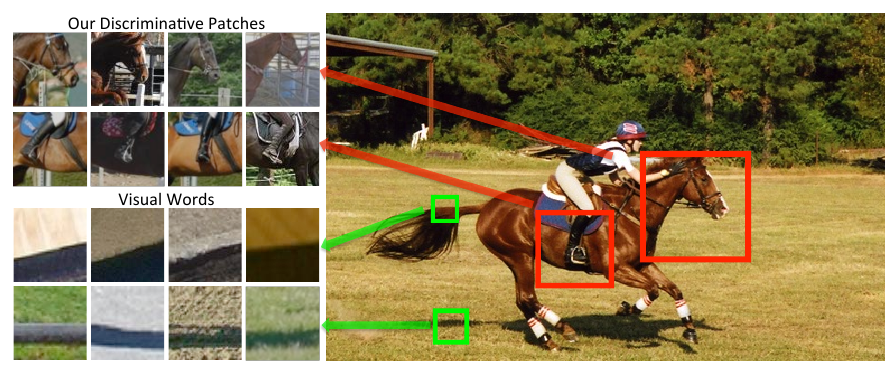
\includegraphics[scale = 0.4]{pics/1_the_idea.png}
\end{figure}
\end{block}

\end{frame}

\begin{frame}
\frametitle{Discriminative Patches}
We want patches that represents the essence of the image, not just its gradients!
\begin{block}{Required properties}
\begin{itemize}
\item Representative
\item Discriminative enough from the rest of the world
\end{itemize}
\end{block}

\end{frame}


\begin{frame}
\frametitle{Motivation}

\begin{block}{Opens doors for further research}
\begin{itemize}
\item More complex classification
\item Scene understanding
\end{itemize}
\end{block}

\begin{block}<2->{Example}
\begin{itemize}
\item What makes Paris look like Paris? \footnote{C.Doersch, et al. What Makes Paris Look like Paris? (SIGGRAPH 2012)}
\end{itemize}
\end{block}

\end{frame}


\begin{frame}
\frametitle{Motivation}

PARIS - NOT PARIS?

\end{frame}



\section{Method}

\begin{frame}
\frametitle{Idea}

Unsupervised learning of "discriminativeness"\\
(without any evidence of humans)

\begin{block}<2->{Basic Process}
\begin{itemize}
\item<2-> Learning patches from the interesting set (discovery set $\mathcal{D}$)
\item<2-> Against the rest of the world (large world set $\mathcal{N}$)
\item<2-> Shared feature space: HOG Descriptor
\item<2-> Unsupervised Learning: k-Means + Support Vector Machine
\item<2-> Determining clusters of the same "visual concept"
\end{itemize}
\end{block}

\end{frame}


\begin{frame}
\frametitle{The Algorithm}

\begin{block}{Pseudocode}
\begin{figure}
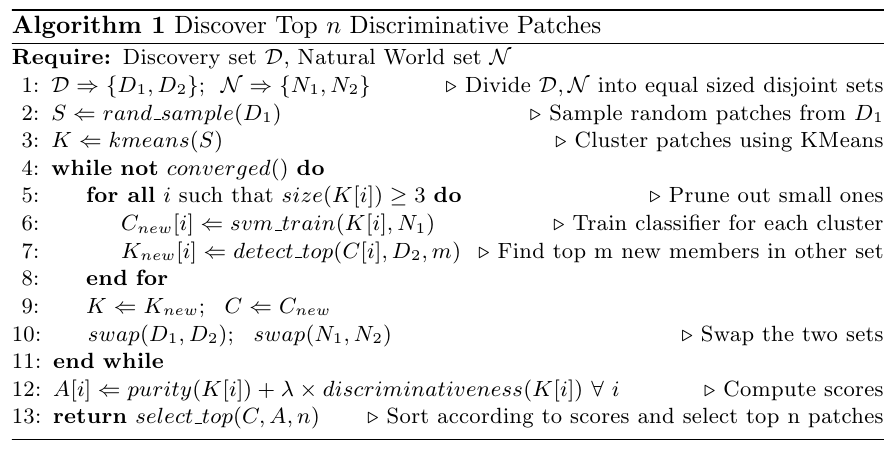
\includegraphics[width= 0.9\textwidth]{pics/algorithm.png}
\end{figure}
\end{block}

\end{frame}

\section{Experiments}


\section{Conclusions}

ihre resultate (im paper): detailreicher

unsere: trotz reduzierter datens�tze gute ergebnisse


\end{document}